\chapter*{} %Property-Based Testing in pure functional ABS
\label{ch:property}

When implementing an Agent-Based Simulation (ABS) it is of fundamental importance that the implementation is correct up to some specification and that this specification matches the real world in some way. This process is called verification and validation (V\&V), where \textit{validation} is the process of ensuring that a model or specification is sufficiently accurate for the purpose at hand whereas \textit{verification} is the process of ensuring that the model design has been transformed into a computer model with sufficient accuracy \cite{robinson_simulation:_2014}. In other words, validation determines if we are we building the \textit{right model}, and verification if we are building the \textit{model right} up to some specification \cite{balci_verification_1998}.

% there is no general validity, an approach is TDD: V&V particularly difficult in ABS
One can argue that ABS should require more rigorous programming standards than other computer simulations \cite{polhill_ghost_2005}. Because researchers in ABS look for an emergent behaviour in the dynamics of the simulation, they are always tempted to look for some surprising behaviour and expect something unexpected from their simulation. 
Also, due to ABS' \textit{constructive / exploratory} nature \cite{epstein_chapter_2006, epstein_generative_2012}, there exists some uncertainty about the dynamics the simulation will produce before running it. The authors \cite{ormerod_validation_2006} see the current process of building ABS as a discovery process where models of an ABS often lack an analytical solution in general, which makes verification much harder if there is no such solution. Thus it is often very difficult to judge whether an unexpected outcome can be attributed to the model or has in fact its roots in a subtle programming error \cite{galan_errors_2009}.

In general this implies that it is not possible to prove that a model is valid in general but that the best we can do is to \textit{raise the confidence} in the correctness of the simulation. Therefore, the process of V\&V is not the proof that a model is correct but the \textit{process} of trying to show that the model is \textit{not incorrect}. The more checks one carries out which show that it is not incorrect, the more confidence we can place on the models validity. To tackle such a problem in software, software engineers have developed the concept of test-driven development (TDD).

Test-Driven Development (TDD) was popularised in the early 00s by Kent Beck \cite{beck_test_2002} as a way to a more agile approach to software-engineering, where instead of doing each step (requirements, implementation, testing,...) as separated from each other, all of them are combined in shorter cycles. Put shortly, in TDD tests are written for each feature before actually implementing it, then the feature is fully implemented and the tests for it should pass. This cycle is repeated until the implementation of all requirements has finished. Traditionally TDD relies on so called unit-tests which can be understood as a piece of code which when run isolated, tests some functionality of an implementation. Thus we can say that test-driven development in general and unit testing together with code-coverage in particular, guarantee the correctness of an implementation to some informal degree, which has been proven to be sufficiently enough through years of practice in the software industry all over the world. 

\medskip

The work \cite{collier_test-driven_2013} was the first to discusses how to apply TDD to ABS, using unit testing to verify the correctness of the implementation up to a certain level. They show how to implement unit-tests within the RePast Framework \cite{north_complex_2013} and make the important point that such a software needs to be designed to be sufficiently modular otherwise testing becomes too cumbersome and involves too many parts. The paper \cite{asta_investigation_2014} discusses a similar approach to DES in the AnyLogic software toolkit. 

The paper \cite{onggo_test-driven_2016} proposes Test Driven Simulation Modelling (TDSM) which combines techniques from TDD to simulation modelling. The authors present a case study for maritime search-operations where they employ ABS. They emphasise that simulation modelling is an iterative process, where changes are made to existing parts, making a TDD approach to simulation modelling a good match. They present how to validate their model against analytical solutions from theory using unit-tests by running the whole simulation within a unit-test and then perform a statistical comparison against a formal specification. %This approach will become of importance later on in our SIR and Sugarscape case studies.

The paper \cite{gurcan_generic_2013} gives an in-depth and detailed overview over verification, validation and testing of agent-based models and simulations and proposes a generic framework for it. The authors present a generic UML class model for their framework which they then implement in the two ABS frameworks RePast and MASON. Both of them are implemented in Java and the authors provide a detailed description how their generic testing framework architecture works and how it utilises unit testing with JUnit to run automated tests. To demonstrate their framework they provide also a case study of an agent-base simulation of synaptic connectivity where they provide an in-depth explanation of their levels of test together with code.

\medskip

% the gap
Although it would be interesting to see how we can apply unit testing to our approach, it is straight forward, nothing new and does not constitute unique research. Thus, in this chapter we introduce an additional technique for TDD: \textit{property-based testing}, which can be seen as complementary to unit testing. Property-based testing has its origins \cite{claessen_quickcheck_2000,claessen_testing_2002,runciman_smallcheck_2008} in Haskell, where it was first conceived and implemented. It has been successfully used for testing Haskell code for years and also been proven to be useful in the industry \cite{hughes_quickcheck_2007}. We show and discuss how this technique can be applied to test pure functional ABS implementations. To our best knowledge property-based testing has never been looked at in the context of ABS and this thesis is the first one to do so.

\medskip

The main idea of property-based testing is to express model-specifications and laws directly in code and test them through \textit{automated} and \textit{randomised} test-data generation. Thus one hypothesis of this thesis is that due to ABS \textit{stochastic} and \textit{exploratory / generative / constructive } nature, property-based testing is a natural fit for testing ABS in general and pure functional ABS implementations in particular. It thus should pose a valuable addition to the already existing testing methods in this field, worth exploring. To substantiate and test our hypothesis, we present two case-studies. First, the agent-based SIR model as introduced in Chapter \ref{sec:sir_model}, which is of explanatory nature, where we show how to express formal model-specifications in property-tests. Second, the SugarScape model as introduced in Chapter \ref{sec:sugarscape}, which is of exploratory nature, where we show how to express hypotheses in property-tests and how to property-test agent functionality. 
%Again, we emphasise that we see it as an addition to TDD, where it works in combination with unit testing to verify and validate a simulation to increase the confidence in its correctness. % and is a useful tool for expressing regression tests.

\medskip

Note that property-based testing has a close connection to model-checking \cite{mcmillan_symbolic_1993}, where properties of a system are proved in a formal way. The important difference is that the checking happens directly on code and not on the abstract, formal model, thus one can say that it combines model-checking and unit testing, embedding it directly in the software-development and TDD process without an intermediary step. We hypothesise that adding it to the already existing testing methods in the field of ABS is of substantial value as it allows to cover a much wider range of test-cases due to automatic data generation. This can be used in two ways: to verify an implementation against a formal specification and to test hypotheses about an implemented simulation. This puts property-based testing on the same level as agent- and system testing, where not technical implementation details of e.g. agents are checked like in unit-tests but their individual complete behaviour and the system behaviour as a whole.

The work \cite{onggo_test-driven_2016} explicitly mentions the problem of test coverage which would often require to write a large number of tests manually to cover the parameter ranges sufficiently enough - property-based testing addresses exactly this problem by \textit{automating} the test-data generation. Note that this is closely related to data-generators \cite{gurcan_generic_2013}, load generators and random testing \cite{burnstein_practical_2010}. Property-based testing though goes one step further by integrating this into a specification language directly into code, emphasising a declarative approach and pushing the generators behind the scenes, making them transparent and focusing on the specification rather than on the data-generation. 

\section*{Property-Based Testing}
\label{sec:proptesting}

Property-based testing allows to formulate \textit{functional specifications} in code which then a property-based testing library tries to falsify by \textit{automatically} generating test-data, covering as much cases as possible. When a case is found for which the property fails, the library then reduces the test-data to its simplest form for which the test still fails e.g. shrinking a list to a smaller size. It is clear to see that this kind of testing is especially suited to ABS, because we can formulate specifications, meaning we describe \textit{what} to test instead of \textit{how} to test. Also the deductive nature of falsification in property-based testing suits very well the constructive and exploratory nature of ABS. Further, the automatic test-generation can make testing of large scenarios in ABS feasible because it does not require the programmer to specify all test-cases by hand, as is required in e.g. traditional unit tests.

Property-based testing was introduced in \cite{claessen_quickcheck_2000,claessen_testing_2002} where the authors present the QuickCheck library in Haskell, which tries to falsify the specifications by \textit{randomly} sampling the test space. We argue, that the stochastic sampling nature of this approach is particularly well suited to ABS, because it is itself almost always driven by stochastic events and randomness in the agents behaviour, thus this correlation should make it straightforward to map ABS to property-testing.
%The main challenge when using QuickCheck, as will be shown later, is to write \textit{custom} test-data generators for agents and the environment which cover the space sufficiently enough to not miss out on important test-cases.
According to the authors of QuickCheck \textit{"The major limitation is that there is no measurement of test coverage."} \cite{claessen_quickcheck_2000}. Although QuickCheck provides help to report the distribution of test-cases it is not able to measure the coverage of tests in general. This could lead to the case that test-cases which would fail are never tested because of the stochastic nature of QuickCheck. Fortunately, the library provides mechanisms for the developer to measure coverage in specific test-cases where the data and its (expected) distribution is known to the developer. This is a powerful tool for testing randomness in ABS as will be shown in subsequent chapters.

\medskip

As a remedy for the potential coverage problems of QuickCheck, there exists also a deterministic property-testing library called SmallCheck \cite{runciman_smallcheck_2008}, which instead of randomly sampling the test-space, enumerates test-cases exhaustively up to some depth. It is based on two observations, derived from model-checking, that (1) \textit{"If a program fails to meet its specification in some cases, it almost always fails in some simple case"} and (2) \textit{"If a program does not fail in any simple case, it hardly ever fails in any case} \cite{runciman_smallcheck_2008}. This non-stochastic approach to property-based testing might be a complementary addition in some cases where the tests are of non-stochastic nature with a search-space  too large to test manually by unit tests but small enough to enumerate exhaustively. The main difficulty and weakness of using SmallCheck is to reduce the dimensionality of the test-case depth search to prevent combinatorial explosion, which would lead to exponential number of cases. Thus one can see QuickCheck and SmallCheck as complementary instead of in opposition to each other.

\subsection*{A brief overview of QuickCheck}
To give a rough idea on how property-based testing works in Haskell, we give a few examples of property-tests on lists, which are directly expressed as functions in Haskell. Such a function has to return a \textit{Bool} which indicates \textit{True} in case the test succeeds or \textit{False} if not and can take input arguments which data is automatically generated by QuickCheck.

\begin{HaskellCode}
-- concatenation operator (++) is associative
append_associative :: [Int] -> [Int] -> [Int] -> Bool
append_associative xs ys zs = (xs ++ ys) ++ zs == xs ++ (ys ++ zs)

-- the reverse of a reversed list is the original list
reverse_reverse :: [Int] -> Bool
reverse_reverse xs = reverse (reverse xs) == xs

-- reverse is distributive over concatenation (++)
-- this test fails for explanatory reasons, for a correct 
-- property xs and ys need to be swapped on the right-hand side!
reverse_distributive :: [Int] -> [Int] -> Bool
reverse_distributive xs ys = reverse (xs ++ ys) == reverse xs ++ reverse ys

-- running the tests
main :: IO ()
main = do
  quickCheck append_associative
  quickCheck reverse_reverse
  quickCheck reverse_distributive
\end{HaskellCode}

When we run the tests using \textit{main}, we get the following output:

\begin{verbatim}
+++ OK, passed 100 tests.
+++ OK, passed 100 tests.
*** Failed! Falsifiable (after 5 tests and 6 shrinks):    
[0]
[1]
\end{verbatim}

We see that QuickCheck generates 100 test-cases for each property-test and it does this by generating random data for the input arguments. Note that we have not specified any data for our input arguments; QuickCheck is able to provide a suitable data-generator through type-inference: for lists and all the existing Haskell types like Int there exist custom generators already.

QuickCheck generates 100 test-cases by default and requires all to pass - if there is a test-case which fails, the overall property-test fails and QuickCheck shrinks the input to a minimal size for which the case still fails and reports it as a counter example. This is the case in the last property-test \textit{reverse\_distributive} which is wrong as \textit{xs} and \textit{ys} need to be swapped on the right-hand side. In this run, QuickCheck found a counter-example to the property after 5 tests and applied 6 shrinks to find the minimal failing example of \textit{xs = [0]} and \textit{ys = [1]}. If we swap \textit{xs} and \textit{ys}, the property-test passes 100 test-cases just like the other two did. Note that it is possible to configure QuickCheck to generate more or less random test-cases, which can be used to increase the coverage if the sampling space is quite large - this will become useful later.

\subsubsection*{Properties and Generators}
TODO: property
TODO: label
TODO: ==>
TODO: generators

\subsubsection*{Coverage}
TODO: cover with checkCoverage


\section*{Testing ABS implementations}
\label{sec:testingABS}
TODO: this is a rather weak section, polish it by writing more general about it and how we can use property-based testing for it. if i cannot come up with something more substantial simply scrap it

Generally we need to distinguish between two types of testing / verification in ABS.

\begin{enumerate}
	\item Testing / verification of models for which we have real-world data or an analytical solution which can act as a ground-truth - examples for such models are the SIR model, stock-market simulations, social simulations of all kind.
	\item Testing / verification of models which are of exploratory nature, inspired by real-world phenomena but for which no ground-truth per se exists - examples for such models is the Sugarscape \cite{epstein_growing_1996} or Agent\_Zero model \cite{epstein_agent_zero:_2014}.
\end{enumerate}

The baseline is that either one has an analytical model as the foundation of an agent-based model or one does not. In the former case, e.g. the SIR model, one can very easily validate the dynamics generated by the simulation to the one generated by the analytical solution through System Dynamics. In the latter case one has basically no idea or description of the emergent behaviour of the system prior to its execution e.g. SugarScape. In this case it is important to have some hypothesis about the emergent property / dynamics. The question is how verification / validation works in this setting as there is no formal description of the expected behaviour: we don't have a ground-truth against which we can compare our simulation dynamics.

One distinguishes between black-box and white-box verification where in white-box verification one looks directly at code and reasons about it whereas in black-box verification one generally feeds input to the software / functions / methods and compares it to expected output. Black-box verification is our primary concern in this chapter as property-based testing is an instance of black-box verification. In the case of ABS we have the following levels of black-box tests \cite{nguyen_testing_2011}: %%Although the work on TDD is scarce in ABS, there exists quite some research on applying TDD and unit testing to multi-agent systems (MAS). Although MAS is a different discipline than ABS, the latter one has derived many technical concepts from the former one, thus testing concepts applied to MAS might also be applicable to ABS. The paper \cite{nguyen_testing_2011} is a survey of testing in MAS. It distinguishes between unit-tests of parts that make up an agent, agent tests which test the combined functionality of parts that make up an agent, integration tests which test the interaction of agents within an environment and observe emergent behaviour, system tests which test the MAS as a system running at the target environment and acceptance test in which stakeholders verify that the software meets their goal. Although not all ABS simulations need acceptance and system tests, still this classification gives a good direction and can be directly transferred to ABS. 
\begin{enumerate}
	\item Isolated and interacting agent behaviour parts - test the individual parts which make up the agent behaviour under given inputs. Also test if interaction between agents are correct. For this we can use traditional unit-tests as shown by \cite{collier_test-driven_2013} and also property-based testing as we will show in the case studies.
	\item Simulation dynamics - compare emergent dynamics of the ABS as a whole under given inputs to an analytical solution or real-world dynamics in case there exists some, using statistical tests. We see this type of tests conceptually as property-tests as well because we are testing properties of the model / simulation as we will see in the case-studies. Technically speaking we can use both unit and property-based tests to implement them - conceptually they are property-tests.
	\item Hypotheses - test whether hypotheses about the model are valid or invalid. This is very similar to the previous point but without comparing it to analytical solutions or real-world dynamics but only to some hypothetical values.
\end{enumerate}

TODO: make it clear that we focus on the event-driven SIR implemention only. why? because of its more interesting nature and because its concepts are also applicable to the sugarscape as well. the time-driven implementation will be shortly discussed in releveant sections.

\chapter{Verifying an explanatory model: \\ The SIR model specification}
\label{ch:prop_explanatory}
As first use-case we discuss how we can use property-based testing to verify the \textit{explanatory} agent-based SIR model as introduced in Chapter \ref{sec:sir_model}. To verify it, we need to make sure it is correct up to some specification. We aim at connecting the agent-based implementation to the SD specification, by formalising it into properties within a property-test. The SD specification can be given through the differential equations shown in Chapter \ref{sec:sir_model}, which we repeat here:

\begin{equation}
\begin{split}
\frac{\mathrm d S}{\mathrm d t} = -infectionRate \\
\frac{\mathrm d I}{\mathrm d t} = infectionRate - recoveryRate \\
\frac{\mathrm d R}{\mathrm d t} = recoveryRate 
\end{split}
\quad
\begin{split}
infectionRate = \frac{I \beta S \gamma}{N} \\
recoveryRate = \frac{I}{\delta} 
\end{split}
\end{equation}
\label{eq:sir_delta_rates}

Solving these equations is done by integrating over time. In the SD terminology, the integrals are called \textit{Stocks} and the values over which is integrated over time are called \textit{Flows}. At $t = 0$ a single agent is infected because if there wouldn't be any infected agents, the system would immediately reach equilibrium - this is also the formal definition of the steady state of the system: as soon as $I(t) = 0$ the system won't change any more.

\begin{align}
S(t) &= N - I(0) + \int_0^t -infectionRate\, \mathrm{d}t \\
I(0) &= 1 \\
I(t) &= \int_0^t infectionRate - recoveryRate\, \mathrm{d}t \\
R(t) &= \int_0^t recoveryRate\, \mathrm{d}t
\end{align}

\section{Deriving the properties}
The key to encode these specifications into a property is to understand that the stocks of \textit{S}, \textit{I} and \textit{R} change \textit{per time-unit} by the given rates. This means that if we run an SD simulation for 1 time-unit, the differences between the S, I and R stocks are the values specified in equations \ref{eq:sir_delta_rates}. %This property has to hold for \textit{any} initial value for S, I and R.

Translating this into a property of our ABS implementation is analogous. We count the number of initially S, I and R agents and run the simulation for 1 time-unit to get new S, I and R numbers. The differences should \textit{average} at the values specified in equations \ref{eq:sir_delta_rates} as well. This property has to hold for \textit{any} agent population. Note that due to ABS stochastic nature it is not enough to run only one replication of the simulation for 1 time-unit but we actually need multiple replications ($> 100$) to get statistically robust results. We then use two-tailed t-tests to compare the expected averages to the actual averages. If all 3 tests pass the whole property-test passes.

\section{Implementing a property-test}
We start by defining the type of our property, which takes a list of \textit{SIRStates} and returns a \textit{Bool}.

\begin{HaskellCode}
prop_sd_rates :: [SIRState] -> Bool
\end{HaskellCode}

Properties in QuickCheck are required to return \textit{Bool} to indicate success or failure - the arguments required for the function are then randomly generated and provided by QuickCheck. For QuickCheck to be able to generate random values of \textit{SIRState} we need to implement an instance of the \textit{Arbitrary} typeclass for \textit{SIRState}. This is straight forward: we \textit{uniformly} pick one out of the 3 possible values.

\begin{HaskellCode}
instance Arbitrary SIRState where
  -- arbitrary :: Gen SIRState
  -- Uniformly pick one of the 3 elements.
  arbitrary = elements [Susceptible, Infected, Recovered]
\end{HaskellCode}

If we want to have a different distribution of the Susceptible, Infected and Recovered states we can also provide a different \textit{Arbitrary} implementation:

\begin{HaskellCode}
instance Arbitrary SIRState where
  -- arbitrary :: Gen SIRState
  -- Susceptible are picked 3 times, Infected 2 times more often than Recovered
  arbitrary = frequency [ (3, return Susceptible)
                        , (2, return Infected)
                        , (1, return Recovered) ]
\end{HaskellCode}

Because we are running replications, we need random seeds to create random-number generators for each replication. We don't make them an argument to the property-test because we don't want to let QuickCheck handle them for us. The reason for that is that if we make it a parameter to the function, QuickCheck tries to vary it as well, meaning that we have less variance and test-cases over the initial population. Thus we generate the seeds manually but relying on QuickChecks random functionality.

\begin{HaskellCode}
prop_sd_rates :: [SIRState] -> Gen Bool
prop_sd_rates as = do
    -- Draw a list of replications random Ints over the full Int range to  
    -- reach maximum variance (reduce probability of drawing identical seeds)
    seeds <- vectorOf replications (choose (minBound, maxBound))
    return (prop_sd_ratesAux seeds)
  where
    prop_sd_ratesAux :: [Int] -> Bool
    prop_sd_ratesAux seeds = allTTestsPass -- see below
\end{HaskellCode}

Next we encode the SD specification as explained above into code.

% NOTE: we omited fromIntegral to make it more readable
\begin{HaskellCode}
-- initial values of S,I and R and total number of agents N
s0 = length (filter (==Susceptible) as)
i0 = length (filter (==Infected) as)
r0 = length (filter (==Recovered) as)
n  = s0 + i0 + r0

-- explicit re-naming
beta  = contactRate
gamma = infectivity
delta = illnessDuration

-- infection-rate
ir = if n == 0 then 0 else (i0 * beta * s0 * gamma) / n
-- recovery-rate 
rr = i0 / delta

-- S value after 1 time-unit 
s = s0 - ir
-- I value after 1 time-unit
i = i0 + (ir - rr)
-- R value after 1 time-unit
r = r0 + rr
\end{HaskellCode}

Then we run replications (100) of the simulation for 1.0 time-unit with same $\Delta t = 0.1$ as in Chapter \ref{sec:timedriven_firststep} to get lists of new S, I and R values.

\begin{HaskellCode}
-- run for 1 time-unit
dur = 1.0
-- same dt as in time-driven chapter implementation
dt = 0.1
-- generate random-number generator for each replication
rngs = map mkStdGen seeds
-- compute simulated values for s, i and r
(ss, is, rs) = unzip (map (last . runSIR dur dt as beta gamma delta) rngs)
\end{HaskellCode}

Finally we run two-tailed t-tests with confidence of 0.95 ($\alpha = 0.05$) for all 3 lists of the new S,I and R values.

% NOTE: tTestSamples return a Maybe Bool but we dont care about that detail here
\begin{HaskellCode}
confidence = 0.95
sTest = tTestSamples TwoTail s (1 - confidence) ss
iTest = tTestSamples TwoTail i (1 - confidence) is
rTest = tTestSamples TwoTail r (1 - confidence) rs

-- property-test passes if all 3 t-tests pass
allTTestsPass = sTest && iTest && rTest
\end{HaskellCode}

\section{Test results}
When testing the property with QuickCheck, by default 100 random test-cases will be generated and \textit{all} have to pass so that the whole property-test passes. Unfortunately, the whole property-test fails - not all 100 random test-cases go through even if we run the whole property-test repeatedly. QuickCheck prints out the random population it generated for the failing random test-case to give a counter-example for the assumption we encoded. Repeated runs show that the counter-examples seem to be lacking any regular pattern like Susceptibles only or 0 Infected - we seem to be failing randomly.

Indeed the fact that we are failing randomly reveals the fundamental difference between SD and ABS: due to ABS' stochastic nature, an ABS cannot match an SD exactly because it is much richer in its dynamics. This enables ABS to explore and reveal paths which are not possible in deterministic SD. In the case of the SIR model, such an alternative path would be the immediate recovery of the single infected agent at the beginning without infecting any other agent. This is not possible in the SD case: in case there is 1 infected agent, the whole epidemic will unfold.

The difficulty of comparing dynamics between SD and ABS and the impracticality to compare them \textit{exactly} was shown by \cite{macal_agent-based_2010} in the case of the SIR model, where the author shows that it is bimodal. Indeed, that is also supported by our observations. When looking at the samples of failed t-tests by plotting them in a histogram, it shows clearly that the values exhibit strong outliers, arriving at a skewed / fat tailed / bimodal histogram. %This means that they are not normally distributed, which is a base assumption and a necessity for t-tests.
The authors \cite{figueredo_comparing_2014} approach the problem of comparing ABS to SD more generally and propose different statistical techniques of how to approach the problem. 
We don't go into further statistical analysis of this problem here as it is not the aim of this thesis but we rather want to see what options we have in pushing the existing approach closer to the SD dynamics, giving us some measure of approximation.

\section{Accepting failure}
The different nature of ABS and SD has the implication that the binary approach of QuickCheck, where the whole property-test fails when a single random test-case fails, is too strict for testing ABS in general and our problem in particular. As a remedy, we can use \textit{maxFailPercent} \footnote{As of the time of writing this thesis (2nd April 2019), this only exists as a pull request \url{https://github.com/nick8325/quickcheck/pull/239} and has not been merged into the main branch of QuickCheck. Thus we use the QuickCheck from \url{https://github.com/stevana/quickcheck/tree/feat/max-failed-percent} who has provided the implementation of \textit{maxFailPercent}.} as a configuration argument to QuickCheck which allows the failure of a given percentage of random-tests cases. The argument behaves in a way that it tries to run up to the 100 default successful random test-cases but fails the overall property-test if the percentage of failed random test-cases is reached. By switching from a binary PASS/FAIL to a more probabilistic measure, reflecting reliability, we have now a tool we can use for measuring the gap between the SD specification and our ABS implementation. Note that a single run is not enough to create robust estimates about failure because QuickCheck always starts out with new seeds. Thus in our experiments, to get a more robust estimate we average 10 runs and report the average with the standard deviation. 

As a first test we run the same property-test again but allow a failure of 100\% to see how many tests will actually pass and how many will fail. In a first estimate run we get: \textit{*** Failed! Passed only 88 tests; 100 failed (53\%) tests}. This means QuickCheck ran 88 successful random test-cases for the property-test before reaching 100\% of failed tests, meaning that out of a total of 173 random test-cases 53\% were failed ones. When averaging 10 runs, 86.1 (4.3) pass with 100 failed tests amounting to a failure percentage of 53.3\% (1.05).
%1. *** Failed! Passed only 88 tests; 100 failed (53%) tests
%2. *** Failed! Passed only 83 tests; 100 failed (54%) tests.
%3. *** Failed! Passed only 86 tests; 100 failed (53%) tests.
%4. *** Failed! Passed only 82 tests; 100 failed (54%) tests.
%5. *** Failed! Passed only 94 tests; 100 failed (51%) tests.
%6. *** Failed! Passed only 88 tests; 100 failed (53%) tests.
%7. *** Failed! Passed only 82 tests; 100 failed (54%) tests.
%8. *** Failed! Passed only 92 tests; 100 failed (52%) tests.
%9. *** Failed! Passed only 82 tests; 100 failed (54%) tests.
%10. *** Failed! Passed only 84 tests; 100 failed (54%) tests.
%[88,83,86,82,94,88,82,92,82,84]
%[53,54,53,54,51,54,54,52,54,54]

\paragraph{Comparison to noise}
To make sure that our approach is going in the right direction at all, we replaced the SIR simulation with a rather simple noise-generator: it generates random values for S, I and R which have to sum up to the size of the population we are comparing against. Indeed, it performs considerably worse than our initial property-test: on average only 19.7 (2.7) tests pass with 100 failed, and a failure percentage of 83\% (1.7). 

%1. *** Failed! Passed only 15 tests; 100 failed (86%) tests.
%2. *** Failed! Passed only 20 tests; 100 failed (83%) tests.
%3. *** Failed! Passed only 23 tests; 100 failed (81%) tests.
%4. *** Failed! Passed only 20 tests; 100 failed (83%) tests.
%5. *** Failed! Passed only 23 tests; 100 failed (81%) tests.
%6. *** Failed! Passed only 20 tests; 100 failed (83%) tests.
%7. *** Failed! Passed only 23 tests; 100 failed (81%) tests.
%8. *** Failed! Passed only 18 tests; 100 failed (84%) tests.
%9. *** Failed! Passed only 17 tests; 100 failed (85%) tests.
%10. *** Failed! Passed only 18 tests; 100 failed (84%) tests.
%
%[15,20,23,20,23,20,23,18,17,18]
%[86,83,81,83,81,83,81,84,85,84]

\paragraph{Optimising $\Delta t$}
As already pointed out in \ref{sub:timedriven_results}, the selection of a sufficiently small $\Delta t$ is crucial and it might be very well the case that the original $\Delta t = 0.1$ we used in our implementation and in Chapter \ref{sub:timedriven_results} is not small enough. 

Indeed, when we half it to $\Delta t = 0.05$, 100 tests pass with 54 (10.3) failing on average, resulting in a failure percentage of 34.4\% (4.2) on average.
%1. +++ OK, passed 100 tests; 39 failed (28%).
%2. +++ OK, passed 100 tests; 48 failed (32%).
%3. +++ OK, passed 100 tests; 49 failed (32%).
%4. +++ OK, passed 100 tests; 65 failed (39%).
%5. +++ OK, passed 100 tests; 68 failed (40%).
%6. +++ OK, passed 100 tests; 46 failed (31%).
%7. +++ OK, passed 100 tests; 55 failed (35%).
%8. +++ OK, passed 100 tests; 55 failed (35%).
%9. +++ OK, passed 100 tests; 69 failed (40%).
%10. +++ OK, passed 100 tests; 46 failed (31%).
%[39,48,49,65,68,46,55,55,69,46]
%[28,32,32,39,40,31,35,35,40,31]

Lowering it to $\Delta t = 0.01$ decreases the failure percentage further with 100 tests passing and failed tests averaging at 15.9 (5.2) with 13.4\% (3.8).
%
%1. +++ OK, passed 100 tests; 25 failed (20%).
%2. +++ OK, passed 100 tests; 16 failed (13%).
%3. +++ OK, passed 100 tests; 25 failed (20%).
%4. +++ OK, passed 100 tests; 10 failed (9%).
%5. +++ OK, passed 100 tests; 10 failed (9%).
%6. +++ OK, passed 100 tests; 15 failed (13%).
%7. +++ OK, passed 100 tests; 14 failed (12%).
%8. +++ OK, passed 100 tests; 14 failed (12%).
%9. +++ OK, passed 100 tests; 15 failed (13%).
%10.+++ OK, passed 100 tests; 15 failed (13%).
%
%[25,16,25,10,10,15,14,14,15,15]
%[20,13,20,9,9,13,12,12,13,13]

Using such a property-based test can be used to find an optimally low $\Delta t$. The optimal $\Delta t$ is the lowest for which sufficiently enough tests go through.

\paragraph{Fixing random population size}
The size of the random population is random itself and we observed coverage of ranges from 0 up to 90. Due to ABS' discrete nature, an increased population size \textit{might} lead to a closer approximation to SD dynamics, which are continuous. When fixing the size of the random population to 100 ($\Delta t = 0.01$) we arrive at 100 passing tests and 35 (6) failed on average with 27.4\% (5.8) failure percentage.

%1. +++ OK, passed 100 tests; 30 failed (23%).
%2. +++ OK, passed 100 tests; 45 failed (31%)
%3. +++ OK, passed 100 tests; 32 failed (24%).
%4. +++ OK, passed 100 tests; 31 failed (23%).
%5. +++ OK, passed 100 tests; 36 failed (26%).
%
%[30,45,32,32,36]
%[23,31,24,23,36]

Fixing the population size leads to more failed tests. The reason for that might be that it is less likely to generate test-cases where the dynamics match exactly e.g. 0 agents of either Susceptible, Infected or Recovered. Still this property-test is not as general as varying also the size of the population.

\paragraph{Increasing confidence}
Another approach would be to increase the confidence in our t-tests e.g. to 99\% ($\alpha = 0.01$). When doing so ($\Delta t = 0.01$), 100 tests will pass and an average of 5.6 (2.9) fail with 4.6\% (2.9) of failure.

%
%1. +++ OK, passed 100 tests; 4 failed (3%).
%2. +++ OK, passed 100 tests; 5 failed (4%).
%3. +++ OK, passed 100 tests; 9 failed (8%).
%4. +++ OK, passed 100 tests; 3 failed (2%).
%5. +++ OK, passed 100 tests; 5 failed (4%).
%6. +++ OK, passed 100 tests; 10 failed (9%).
%7. +++ OK, passed 100 tests; 8 failed (7%).
%8. +++ OK, passed 100 tests; 2 failed (1%).
%9. +++ OK, passed 100 tests; 8 failed (7%).
%10 +++ OK, passed 100 tests; 2 failed (1%).
%
%[4,5,9,3,5,10,8,2,8,2]
%[3,4,8,2,4,9,7,1,7,1]

Although it seems that we have finally found a test configuration with a sufficiently low percentage of failure, changing the confidence can be problematic though. By increasing it we lower the risk of rejecting a test which matches the SD dynamics (type I error). On the other hand increasing the confidence also increases the risk of not rejecting tests which do not match the SD dynamics (type II error). 

\paragraph{Comparison to event-driven implementation}
We also implemented this property-test for our event-driven SIR implementation from Chapter \ref{sec:eventdriven_sir}. It has the main advantage that it does not suffer from the sampling issues of the time-driven approach and thus does not require the selection of an optimal $\Delta t$.
The results match on average the ones from the time-driven approach. Running it normally roughly matches the dynamics of $\Delta t = 0.01$, a fixed population size of 100 also matches the time-driven approach with a random population of size 100 and $\Delta t = 0.01$. Further we also got the same results when increasing confidence to 99\% ($\alpha = 0.01$) as in the time-driven approach.

%1. +++ OK, passed 100 tests; 25 failed (20%).
%2. +++ OK, passed 100 tests; 22 failed (18%).
%3. +++ OK, passed 100 tests; 26 failed (20%).
%4. +++ OK, passed 100 tests; 15 failed (13%).
%5. +++ OK, passed 100 tests; 29 failed (22%).
%6. +++ OK, passed 100 tests; 12 failed (10%).
%7. +++ OK, passed 100 tests; 17 failed (14%).
%8. +++ OK, passed 100 tests; 16 failed (13%).
%9. +++ OK, passed 100 tests; 13 failed (11%).
%10. +++ OK, passed 100 tests; 14 failed (12%).
%
%[25,22,26,15,29,12,17,16,13,14]
%>> mean (x)
%ans =  18.900
%>> std (x)
%ans =  6.0818

%TODO: what about using a fixed size random population instead of random size random population? this should increase the smoothness when always using e.g. 1000 or 10.000
%1. +++ OK, passed 100 tests; 30 failed (23%).
%2. +++ OK, passed 100 tests; 29 failed (22%).
%3. +++ OK, passed 100 tests; 44 failed (30%).
%4. +++ OK, passed 100 tests; 40 failed (28%).
%5. +++ OK, passed 100 tests; 41 failed (29%).
%6. +++ OK, passed 100 tests; 41 failed (29%).
%7. +++ OK, passed 100 tests; 38 failed (27%).
%8. +++ OK, passed 100 tests; 36 failed (26%).
%9. +++ OK, passed 100 tests; 30 failed (23%).
%10. +++ OK, passed 100 tests; 46 failed (31%).
%
%[30,29,44,40,41,41,38,36,30,46]
%>> mean (x)
%ans =  37.500
%>> std (x)
%ans =  6.0782

%TODO: confidence 0.99
%1. +++ OK, passed 100 tests; 6 failed (5%).
%2. +++ OK, passed 100 tests; 5 failed (4%).
%3. +++ OK, passed 100 tests; 7 failed (6%).
%4. +++ OK, passed 100 tests; 1 failed (0%).
%5. +++ OK, passed 100 tests; 5 failed (4%).
%6. +++ OK, passed 100 tests; 6 failed (5%).
%7. +++ OK, passed 100 tests; 6 failed (5%).
%8. +++ OK, passed 100 tests; 5 failed (4%).
%9. +++ OK, passed 100 tests; 10 failed (9%).
%10. +++ OK, passed 100 tests; 6 failed (5%).
%
%[6,5,7,1,5,6,6,5,10,6]
%>> mean (x)
%ans =  5.7000
%>> std (x)
%ans =  2.2136

This is a \textit{strong} indication, that although their underlying implementation technique is different, both implementations produce qualitatively same dynamics. It would be interesting to compare both implementations on using property-based testing, using an unpaired two-tailed t-test. We leave this for further research.

\section{Discussion}
By using QuickCheck, we showed how to connect the ABS implementation to the SD specification by deriving a property, based on the SD specification. This property is directly expressed in code and tested through generating random test-cases with random agent populations. We assumed that the underlying SIR implementation, more specific, that all agent behaviour, is correct - we explore testing of individual agent behaviour in the later chapters.

Although our initial idea of matching the ABS implementation to the SD specifications has not worked out in an exact way, we still showed a way of formalizing and expressing these relations in code and testing them using QuickCheck. By allowing failure in our tests using the \textit{maxFailPercent} parameter, we confirmed the importance of selecting an optimal $\Delta t$ as already pointed out in Chapter \ref{sub:timedriven_results}. By having measure of failure, we can use a property-test also as a way of systematically searching for the smallest optimal $\Delta t$, relieving us from making conservative guesses. For the event-driven implementation, there is no such issue and we have verified that it produces qualitatively the same results.

The results showed that the ABS implementation comes close to the original SD specification but does not match it exactly - it is indeed richer in its dynamics as \cite{macal_agent-based_2010, figueredo_comparing_2014} have already shown. Our approach might work out better for a different model, which has a better behaved underlying specification than the bimodal SIR. % for which a proper statistical analysis is not the aim and focus of this thesis is left for other researchers to dwell upon.

\chapter{Verifying an exploratory model: \\ Hypotheses in Sugarscape}
\label{ch:prop_exploratory}

In this chapter we look at how property-based testing can be made of use to verify the \textit{exploratory} Sugarscape model \cite{epstein_growing_1996} as already introduced in Chapter \ref{sec:sugarscape}. Whereas in the previous chapter on testing the explanatory SIR case-study we had an analytical solution, the fundamental difference in the exploratory Sugarscape model is that none such analytical solutions exist. This raises the question, which properties we can actually test in such a mode.

The answer lies in the very nature of exploratory models: they exist to explore and understand phenomena of the real world. Researchers come up with a model to explain the phenomena and then (hopefully) come up with a few questions and  \textit{hypotheses} about the emergent properties. The actual simulation is then used to test and refine the hypotheses. Indeed, descriptions, assumptions and hypotheses of varying formal degree are abound in the Sugarscape model. Examples are: \textit{the carrying capacity becomes stable after 100 steps; when agents trade with each other, after 1000 steps the standard deviation of trading prices is less than 0.05; when there are cultures, after 2700 steps either one culture dominates the other or both are equally present}. 

We show how to use property-testing to formalise and check such hypotheses. For this purpose we undertook a full \textit{verification} of our implementation \footnote{The code can be accessed freely from \url{https://github.com/thalerjonathan/phd/tree/master/public/towards/SugarScape/sequential}} from Chapter \ref{sec:sugarscape}. We validated it against the book \cite{epstein_growing_1996} and a NetLogo implementation \cite{weaver_replicating_2009} \footnote{\url{https://www2.le.ac.uk/departments/interdisciplinary-science/research/replicating-sugarscape}}. A longer report on the details of this validation process is attached as Appendix \ref{app:validating_sugarscape}, in this section we focus on QuickChecks role in this process.

The property we test for is whether \textit{the emergent property / hypothesis under test is stable under replicated runs} or not. To put it more technical, we use QuickCheck to run multiple replications with the same configuration but with different random-number streams and require that the tests all pass. During the verification process described in Appendix \ref{app:validating_sugarscape} we have derived and implemented property-tests for the following hypotheses:

\begin{enumerate}
	\item Disease Dynamics all recover - When disease are turned on, if the number of initial diseases is 10, then the population is  able to rid itself completely from all disease within 100 ticks. 
	
	\item Disease Dynamics minority recover - When disease are turned on, if the number of initial diseases is 25, the population is not able to rid itself completely from all diseases within 1,000 ticks.
	
	\item Trading Dynamics - When trading is enabled, the trading prices stabilise after 1,000 ticks with the standard deviation of the prices having dropped below 0.05.
	
	\item Cultural Dynamics - When having two cultures, red and green, after 2,700 ticks, either the red or the blue culture dominates or both are equally strong. If they dominate they make up 95\% of all agents, if they are equally strong they are both within 45\% - 55\%.
	
	\item Inheritance Gini Coefficient - When agents reproduce and can die of age then inheritance of their wealth leads to an unequal wealth distribution measured using the Gini Coefficient \textit{averaging} at 0.35. 

	\item Carrying Capacity - When agents don't mate nor can die from age (chapter II), due to the environment, there is an \textit{average} maximum carrying capacity of agents the environment can sustain. The capacity should be reached after 100 ticks and should be stable from then on.
		
	\item Terracing - When resources regrow immediately, after a few steps the simulation becomes static. Agents will stay on their terraces and will not move any more because they have found the best spot due to their behaviour. About 45\% will be on terraces and 95\% - 100\% are static and not moving any more.
\end{enumerate}

\section{Implementation}
To implement this, we make use of QuickChecks \textit{Generator} concept. A \textit{Generator} defines how specific (random) data can be generated and is implemented using the \textit{Gen} monad where all of QuickChecks random distribution functionality is available. Thus it is only natural that we implement a \textit{Generator} to produce output from a Sugarscape simulation. The generator takes the number of ticks and the scenario with which to run the simulation and returns a list of outputs, one for each tick.

\begin{HaskellCode}
sugarscapeUntil :: Int -> SugarScapeScenario -> Gen [SimStepOut]
sugarscapeUntil ticks params = do
  -- draw a seed for the random-number generator from the full range of Int
  seed <- choose (minBound, maxBound)
  -- create a random-number generators
  let g = mkStdGen seed
  -- initialise the simulation state with the given random-number generator
  -- and the parameters
  let (simState, _, _) = initSimulationRng g params
  -- run the simulation with the given state for number of ticks
  return (simulateUntil ticks simState)
\end{HaskellCode}

Using this generator, we can very conveniently produce sugarscape data within a property. Depending on the problem, we can generate only a single run or multiple replications, in case the hypothesis is assuming \textit{averages}. To see its use, we show the encoding of the \textit{Disease Dynamics (1)} hypothesis. Its type is \textit{Property}, which is required by QuickChecks top-level testing function. To generate a property, the \textit{property} function is used which takes a \textit{Gen Bool} computation or a simple \textit{Bool} function as predicate to indicate success (True) or failure (False). In this case we use a \textit{Gen Bool} to be able to run the sugarscape data generator.

\begin{HaskellCode}
prop_disease_allrecover :: Property
prop_disease_allrecover = property (do
  -- after 100 ticks...
  let ticks  = 100
  -- ... given Animation V-1 parameter configuration ...
  let params = mkParamsAnimationV_1

  -- ... from 1 sugarscape simulation ...
  aos <- sugarscapeLast ticks params
  -- ... counting all infected agents ...
  let infected = length (filter (==False)) map (null . sugObsDiseases . snd) aos
  -- ... should result in all agents to be recovered
  return (infected == 0))
\end{HaskellCode}

QuickCheck runs multiple replications of a property when testing it, where the number is 100 by default. From the implementation it becomes clear, that this hypothesis states that the property has to hold \textit{for all} replications. The \textit{Inheritance Gini Coefficient (5)} hypothesis on the other hand assumes that the Gini Coefficient \textit{averages} at 0.35. We cannot average over replicated runs of the same property thus we have no other option to do the process of averaging within the property. We force this property to be run only \textit{once} but we generate multiple replications of the sugarscape data within the property and employ a two-sided t-test to test the hypothesis. Here is how we encode this into a property-test:

\begin{HaskellCode}
prop_gini :: Int -> Double -> Property
prop_gini repls confidence = once (do
  -- after 1000 ticks...
  let ticks = 1000
  -- ... the gini coefficient should average at 0.35 ...
  let expGini = 0.35
  -- ... given the Figure III-7 parameter configuration ...
  let params = mkParamsFigureIII_7
  
  -- ... from repls replciations ... 
  gini <- vectorOf repls (genGiniCoeff ticks params)

  -- on a two-tailed t-test with given confidence
  let giniTTest = tTestSamples TwoTail expGini (1 - confidence) gini

  return giniTTest)
  
genGiniCoeff :: Int -> SugarScapeScenario -> Gen Double
genGiniCoeff ticks params = do
  -- generate sugarscape data
  aos <- sugarscapeUntil ticks params
  -- extract wealth of the agents in the last step
  let agentWealths = map (sugObsSugLvl . snd) (last aos)
  -- compute gini coefficient and return it
  return (giniCoeff agentWealths)
\end{HaskellCode}

\section{Running the tests}
As already pointed out, QuickChec by default tries to run up 100 replications of a \textit{Property}. If for all 100 replications the predicate evaluates to \textit{True} the property-test succeeds. On the other hand, QuickCheck will stop at the first predicate which evalutes to \textit{False} and marks this property-test as failed. When running all property-tests, this leaves us with the question: \textit{Will they go through?}.

Due to the long time even 1,000 ticks can take to compute, we reduce the number of maximum successful replications required to 10 and indeed when we run it, we are happy: \textit{All went through!}. 

It is important to understand that QuickCheck is always initialised with a new random-number seed when run, thus we might have just been lucky. Indeed,when we run it again, we are not so lucky, and the following hypotheses fail:

Trading Dynamics
Cultural Dynamics

The hypotheses which went through were:
Disease Dynamics all recover
Disease Dynamics no recover

\subsection{Allowing failure}
It is arguably the case that the binary approach of QuickCheck, where the whole property-test fails when a single replication fails, is too strict for testing ABS in general and our hypotheses in particular. The reason for that is, that due to ABS stochastic nature, the hypotheses might hold for a large number of replications but not strictly for all.

As a remedy, we can use \textit{maxFailPercent} \footnote{As of the time of writing this thesis (2nd April 2019), this only exists as a pull request \url{https://github.com/nick8325/quickcheck/pull/239} and has not been merged into the main branch of QuickCheck. Thus we use the QuickCheck from \url{https://github.com/stevana/quickcheck/tree/feat/max-failed-percent} who has provided the implementation of \textit{maxFailPercent}.} as a configuration argument to QuickCheck, which allows the failure of a given percentage of replications. The argument behaves in a way that it tries to run up to the 100 default (or whatever the configuration is) successful replications but fails the overall property-test if the percentage of failed replications is reached. By switching from a binary PASS/FAIL to a more probabilistic measure, reflecting reliability, we have now a more appropriate tool for testing the suitability of our hypotheses. 

We run the tests again with 10 replications each but now allowing 100\% of failure in each case to see how reliable each hypothesis is. In one specific run we get the following result:

\begin{enumerate}
	\item Disease Dynamics all recover: \textit{+++ OK, passed 10 tests.}

	\item Disease Dynamics minority recover: \textit{+++ OK, passed 10 tests.}
		
	\item Trading Dynamics: \textit{+++ OK, passed 10 tests; 2 failed (16\%).} \\ In total 12 tests (replications) were run, out of which 2 failed, which is a 16\% failure rate.
	
	\item Cultural Dynamics: \textit{+++ OK, passed 10 tests; 3 failed (23\%).} \\ In total 13 tests (replications) were run, out of which 3 failed, which is a 23\% failure rate.

	\item Inheritance Gini Coefficient: 
	
	\item Carrying Capacity:
		
	\item Terracing:
\end{enumerate}

How to deal with the failure of the hypotheses is obviously highly model specific. A first approach is to increase the number of replications to run to 100 to get a more robust estimate of the failure rate. If the failure rate stays within reasonable ranges then one can arguably assume that the hypothesis is valid for sufficiently enough cases. On the other hand, if the failure rate escalates, then it is reasonable to deem the hypothesis invalid and refine it or even abandon it altogether. In the hypotheses we presented here we accept the failure rate and even though there the hypotheses fail in some cases, we deem them sufficiently valid for the task at hand.

Note that we disabled shrinking for hypothesis testing as it has no meaning here. The only thing which would be shrunk would be the seed of the random-number generator, which has no intrinsic meaning.

\section{Discussion}
In this chapter we showed how to use QuickCheck to formalise and check hypotheses about an \textit{exploratory} agent-based model, in which no ground truth exists. Due to ABS stochastic nature in general it became obvious that to get a good measure of a hypotheses validity we need to allow failure using the \textit{maxFailPercent} argument of QuickCheck. This allowed us to show that the hypotheses we have presented are sufficiently valid for the task at hand and can indeed be used for expressing and formalising emergent properties of the model and also as regression tests within a TDD cycle.

\section{Case Study II: Sugarscape}
\label{sec:sugarscape_concurrent}
The second case study is the Sugarscape model as introduced in Chapter \ref{sec:sugarscape}. In this case study we look into the potential performance improvement in a model with much more complex agent behaviour and dramatically increased writes on the shared environment.

We implemented the \textit{Carrying Capacity} (p. 30) section of Chapter II of the Sugarscape book \cite{epstein_growing_1996}. In each step agents search (move) to the cell with the most sugar they see within their vision, harvest all of it from the environment and consume sugar because of their metabolism. Sugar regrows in the environment over time. Only one agent can occupy a cell at a time. Agents don't age and cannot die from age. If agents run out of sugar due to their metabolism, they die from starvation and are removed from the simulation. The authors report that the initial number of agents quickly drops and stabilises around a level depending on the model parameters. This is in accordance with our results as we show in Chapter \ref{ch:property} and guarantees that we don't run out of agents. The model parameters are as follows:

\begin{itemize}
	\item Sugar Endowment: each agent has an initial sugar endowment randomly uniform distributed between 5 and 25 units;
	\item Sugar Metabolism: each agent has a sugar metabolism randomly uniform distributed between 1 and 5;
	\item Agent Vision: each agent has a vision randomly uniform distributed between 1 and 6, same for each of the 4 directions (N, W, S, E);
	\item Sugar Growback: sugar grows back by 1.0 unit per step until the maximum capacity of a cell is reached;
	\item Agent Number: initially 500 agents;
	\item Environment Size: 50 x 50 cells with toroid boundaries which wrap around in both x and y dimension.
\end{itemize}

Note that in this implementation (as in the full Chapter II of the book), no direct and no synchronous agent-interactions as we implemented them in Chapter \ref{sec:eventdriven_implementation} are happening. As in the SIR example, all agents interact with each other indirectly through the shared environment. This allows us to regard the implementation as a time-driven, parallel one wherein each step agents act conceptually at the same time.

We compare four different implementations \footnote{The code is freely available at \url{https://github.com/thalerjonathan/phd/tree/master/public/stmabs/code/SugarScape}}:

\begin{enumerate}
	\item Sequential - All agents are run after another (including the environment) and the environment is shared amongst the agents using a \textit{StateT} transformer.
	\item Lock-Based - All agents are run concurrently in the \textit{IO} monad and the environment is shared between the agents, using an \textit{IORef} with the access synchronised through an \textit{MVar} lock.
	\item STM TVar - All agents are run concurrently in the \textit{STM} monad and the environment is shared using a \textit{TVar} between the agents.
	\item STM TArray - All agents are run concurrently in the \textit{STM} monad and the environment is shared using a \textit{TArray} between the agents. 
\end{enumerate}

We follow \cite{lysenko_framework_2008} and measure the average number of steps per second of the simulation over 60 seconds. For each experiment we conducted 8 runs on our machine (see Table \ref{tab:machine_specs}) under no additional work-load and report the average. In the experiments we varied the number of cores when running concurrently - the numbers are always indicated clearly.

%\paragraph{Output} Note that we omit the graphical rendering in the functional approach because it is a serious bottleneck taking up substantial amount of the simulation time. Although visual output is often important in ABS, it is not what we are interested here thus we completely omit it and only output the number of agents in the simulation at each step piped into a file, thus omitting slow output to the console \footnote{Note that we need to produce \textit{some} output because of Haskells laziness - if we wouldn't output anything from the simulation then the expressions would actually never be fully evaluated thus resulting in high number of steps per second but which obviously don't really reflect the true computations done.}.

\paragraph{Ordering} The model specification requires to shuffle agents before every step (Footnote 12 on page 26 \cite{epstein_growing_1996}). In the \textit{Sequential} approach we do this explicitly but in the \textit{Lock-Based} and both \textit{STM} approaches we assume this to happen automatically due to race-conditions in concurrency, thus we arrive at an effectively shuffled processing of agents: we implicitly assume that the order of the agents is \textit{effectively} random in every step. The important difference between the two approaches is that in the \textit{Sequential} approach we have full control over this randomness but in the \textit{STM} not - also this means that repeated runs with the same initial conditions might lead to slightly different results. 
This decision leaves the execution order of the agents ultimately to Haskell's Runtime System and the underlying OS. We are aware that by doing this, we make assumptions that the threads run uniformly distributed (fair) but such assumptions should not be made in concurrent programming. As a result we can expect this fact to produces non-uniform distributions of agent runs but we assumed that for this model this does not has a significance influence - in case of doubt, we could resort to shuffling the agents before running them in every step. We agree that this very problem would deserve in-depth research on its own, where also the influence of non-deterministic ordering on the correctness and results of ABS has to be analysed. This is not the main interest of this section though and we leave it for further research as it is completely beyond the focus of this thesis.

%Note that in the concurrent implementations we have two options for running the environment: either asynchronously as a concurrent agent at the same time with the population agents or synchronously after all agents have run. We must be careful though as running the environment as a concurrent agent can be seen as conceptually wrong because the time when the regrowth of the sugar happens is now completely random. In this case it could happen that sugar regrows in the very first transaction or in the very last, different in each step, which can be seen as a violation of the model specifications. Thus we do not run the environment concurrently with the agents but synchronously after all agents have run.

\subsection{Constant Agent Size}
In a first approach we compare the performance of all implementations on varying numbers of cores. The results are reported in Table \ref{tab:varying_cores} and plotted in Figure \ref{fig:varying_cores}. 

\begin{table}
	\centering
	\begin{tabular}{cc|c|c}
		\multicolumn{1}{ c||  }{\multirow{2}{*}{} } &
		\multicolumn{1}{ |c| }{Cores} & Steps & Retries      \\ \hline \hline 
		
		\multicolumn{1}{ c||  }{\multirow{1}{*}{Sequential} } &
		\multicolumn{1}{ |c| }{1} & 39.4 & N/A     \\ \hline \hline 
		
		\multicolumn{1}{ c||  }{\multirow{4}{*}{Lock-Based} } &
		\multicolumn{1}{ |c| }{1} & 43.0 & N/A       \\ \cline{2-4}
		\multicolumn{1}{ c||  }{}                       &
		\multicolumn{1}{ |c| }{2} & 51.8 & N/A   \\ \cline{2-4}
		\multicolumn{1}{ c||  }{}                       &
		\multicolumn{1}{ |c| }{3} & 57.4 & N/A   \\ \cline{2-4}
		\multicolumn{1}{ c||  }{}                       &
		\multicolumn{1}{ |c| }{4} & 58.1 & N/A   \\ \hline \hline 
		
		\multicolumn{1}{ c||  }{\multirow{4}{*}{STM \textit{TVar}} } &
		\multicolumn{1}{ |c| }{1} & \textbf{47.3} & 0.0       \\ \cline{2-4}
		\multicolumn{1}{ c||  }{}                       &
		\multicolumn{1}{ |c| }{2} & 53.5 & 1.1    \\ \cline{2-4}
		\multicolumn{1}{ c||  }{}                       &
		\multicolumn{1}{ |c| }{3} & 57.1 & 2.2    \\ \cline{2-4}
		\multicolumn{1}{ c||  }{}                       &
		\multicolumn{1}{ |c| }{4} & 53.0 & 3.2   \\ \hline \hline 
		
		\multicolumn{1}{ c||  }{\multirow{4}{*}{STM \textit{TArray}} } &
		\multicolumn{1}{ |c| }{1} & 45.4 & 0.0       \\ \cline{2-4}
		\multicolumn{1}{ c||  }{}                       &
		\multicolumn{1}{ |c| }{2} & \textbf{65.3} & 0.02   \\ \cline{2-4}
		\multicolumn{1}{ c||  }{}                       &
		\multicolumn{1}{ |c| }{3} & \textbf{75.7} & 0.04    \\ \cline{2-4}
		\multicolumn{1}{ c||  }{}                       &
		\multicolumn{1}{ |c| }{4} & \textbf{84.4} & 0.05   \\ \hline \hline 
	\end{tabular}  	
  	
  	\caption{Steps per second and retries on 50x50 grid with 500 initial agents on varying cores.}
	\label{tab:varying_cores}
\end{table}

\begin{figure}
	\centering
	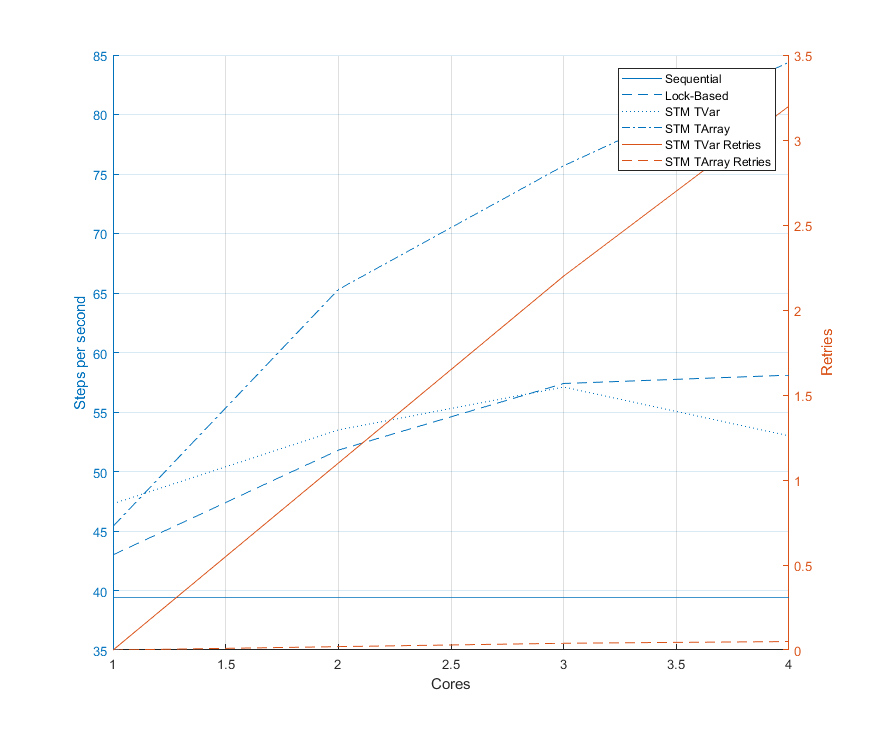
\includegraphics[width=0.7\textwidth, angle=0]{./fig/concurrentabs/sugarscape/varying_cores.png}
	\caption{Steps per second and retries on 50x50 grid and 500 initial agents on varying cores.}
	\label{fig:varying_cores}
\end{figure}

As expected, the \textit{Sequential} implementation is the slowest, followed by the \textit{Lock-Based} and \textit{TVar} approach whereas \textit{TArray} is the best performing one.

We clearly see that using a \textit{TVar} to share the environment is a very inefficient choice in this model: \textit{every} write to a cell leads to a retry independent whether the reading agent reads that changed cell or not, because the data-structure can not distinguish between individual cells. By using a \textit{TArray} we can avoid the situation where a write to a cell in a far distant location of the environment will lead to a retry of an agent which never even touched that cell. Also the \textit{TArray} seems to scale up by 10 steps per second for every core added. It will be interesting to see how far this could go with the Amazon experiment, as we seem not to hit a limit with 4 cores yet.

The inefficiency of \textit{TVar} is also reflected in the nearly similar performance of the \textit{Lock-Based} implementation which even outperforms it on 4 cores. This is due to very similar approaches because both operate on the whole environment instead of only the cells as \textit{TArray} does. This seems to be a bottleneck in \textit{TVar} reaching the best performance on 3 cores, which then drops on 4 cores due to an increasing retries ratio. The \textit{Lock-Based} approach seems to reduce its returns on increased number of cores hitting a limit at 4 cores as well.

\subsection{Scaling up Agents}
So far we kept the initial number of agents at 500, which due to the model specification, quickly drops and stabilises around 200 due to the carrying capacity of the environment as described in the book \cite{epstein_growing_1996} section \textit{Carrying Capacity} (p. 30).

We now want to measure the performance of our approaches under increased number of agents. For this we slightly change the implementation: always when an agent dies it spawns a new one which is inspired by the ageing and birthing feature of Chapter III in the book \cite{epstein_growing_1996}. This ensures that we keep the number of agents roughly constant (still fluctuates but doesn't drop to low levels) over the whole duration. This ensures a constant load of concurrent agents interacting with each other and demonstrates also the ability to terminate and create concurrent agents (threads) dynamically during the simulation.

Except for the \textit{Sequential} approach we ran all experiments with 4 cores (TVar with 3 as well). We looked into the performance of 500, 1,000, 1,500, 2,000 and 2,500 (maximum possible capacity of the 50x50 environment). The results are reported in Table \ref{tab:state_results_agentsscale_time} and plotted in Figure \ref{fig:state_results_agentsscale_time}.

\begin{table}
	\centering
  	\begin{tabular}{ c || c | c | c | c | c }
        Agents  & Sequential & Lock-Based & TVar (3 cores) & TVar (4 cores) & TArray  \\ \hline \hline 
    	    500     & 14.4       & 20.2		  &	20.1           & 18.5       	& \textbf{71.9}    \\ \hline
   		1,000   & 6.8        & 10.8 	      & 10.4           & 9.5         & \textbf{54.8}    \\ \hline
   		1,500   & 4.7        & 8.1 		  & 7.9            & 7.3			& \textbf{44.1}    \\ \hline
   		2,000   & 4.4        & 7.6 		  & 7.4            & 6.7    		& \textbf{37.0}    \\ \hline 
   		2,500   & 5.3        & 5.4 		  & 9.2            & 8.9			& \textbf{33.3}    \\ \hline \hline
   	\end{tabular}
  	
  	\caption{Steps per second on 50x50 grid with varying number of agents with 4 (and 3) cores except Sequential (1 core).}
	\label{tab:state_results_agentsscale_time}
\end{table}

\begin{figure}
	\centering
	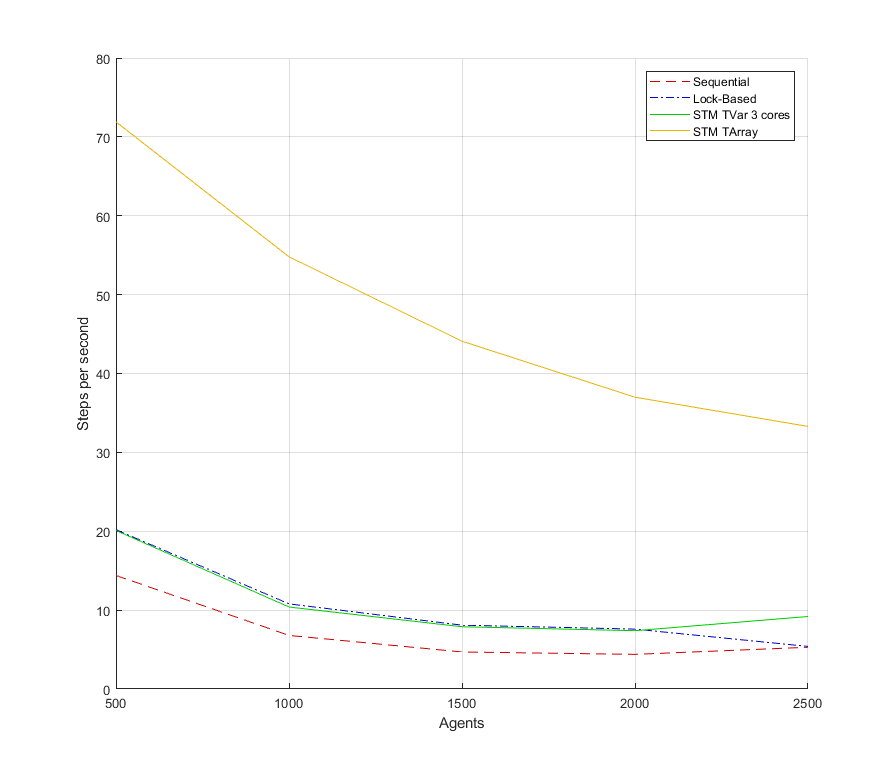
\includegraphics[width=1.0\textwidth, angle=0]{./fig/concurrentabs/sugarscape/varying_agents.png}
	\caption{Steps per second on 50x50 grid and varying number of agents with 4 (and 3) cores except Sequential (1 core).}
	\label{fig:state_results_agentsscale_time}
\end{figure}

As expected, the \textit{TArray} implementation outperforms all others substantially. Also as expected, the \textit{TVar} implementation on 3 cores is faster than on 4 cores as well when scaling up to more agents. The \textit{Lock-Based} approach performs about the same as the \textit{TVar} on 3 cores because of the very similar approaches: both access the \textit{whole} environment. Still the \textit{TVar} approach uses one core less to arrive at the same performance, thus strictly speaking outperforming the \textit{Lock-Based} implementation.

What seems to be very surprising is that in the \textit{Sequential} and \textit{TVar} cases the performance with 2,500 agents is \textit{better} than the one with 2,000 agents. The reason for this is that in the case of 2,500 agents, an agent can't move anywhere because all cells are already occupied. In this case the agent won't rank the cells in order of their pay-off (max sugar) to move to but just stays where it is. We hypothesize that due to Haskells laziness the agents actually never look at the content of the cells in this case but only the number which means that the cells themselves are never evaluated which further increases performance. This leads to the better performance in case of \textit{Sequential} and \textit{TVar} because both exploit laziness.
In the case of the \textit{Lock-Based} approach we still arrive at a lower performance because the limiting factor are the unconditional locks. In the case of the \textit{TArray} approach we also arrive at a lower performance because it seems that STM perform reads on the neighbouring cells which are not subject to lazy evaluation. In Haskell it is notoriously difficult to reason about efficiency (see Chapter \ref{ch:drawbacks} for a short discussion on drawbacks) and this behaviour of improved performance due to Haskells lazyness is no exception. We leave an in-depth investigation for further research as it is beyond the focus of this chapter.

We also measured the average retries both for \textit{TVar} and \textit{TArray} under 2,500 agents where the \textit{TArray} approach shows best scaling performance with 0.01 retries whereas \textit{TVar} averages at 3.28 retries. Again this can be attributed to the better transactional data-structure which reduces retry-ratio substantially to near-zero levels.

\subsection{Going Large-Scale}
To test how far we can scale up the number of cores in both the \textit{Lock-Based} and \textit{TArray} cases, we ran the two experiments (carrying capacity and rebirthing) on Amazon EC2 instances with increasing number of cores starting with 16 and 32 to see if we run into decreasing returns. The results are reported in Table \ref{tab:sug_varying_cores_amazon}.

\begin{table}
	\centering
%  	\begin{tabular}{ c || c | c | c }
%                   & Cores & Carrying Capacity & Rebirthing  \\ \hline \hline 
%    	Lock-Based & 16    & 53.9              & 4.4         \\ \hline
%    	Lock-Based & 32    & 44.2              & 3.6         \\ \hline \hline 
%   		
%   		STM TArray & 16    & \textbf{116.8} (0.23)      & \textbf{39.5} (0.08) \\ \hline
%   		STM TArray & 32    & 109.8 (0.41)      & 31.3 (0.18) \\ \hline \hline 
%   	\end{tabular}
  	
	\begin{tabular}{cc|c|c}
		\multicolumn{1}{ c||  }{\multirow{2}{*}{} } &
		\multicolumn{1}{ |c| }{Cores} & Carrying Capacity    & Rebirthing       \\ \hline \hline 
		
		\multicolumn{1}{ c||  }{\multirow{2}{*}{Lock-Based} } &
		\multicolumn{1}{ |c| }{16} & 53.9              & 4.4       \\ \cline{2-4}
		\multicolumn{1}{ c||  }{}                       &
		\multicolumn{1}{ |c| }{32} & 44.2              & 3.6      \\ \hline \hline 
		
		\multicolumn{1}{ c||  }{\multirow{2}{*}{STM TArray} } &
		\multicolumn{1}{ |c| }{16} & \textbf{116.8} (0.23)      & \textbf{39.5} (0.08)       \\ \cline{2-4}
		\multicolumn{1}{ c||  }{}                       &
		\multicolumn{1}{ |c| }{32} & \textbf{109.8} (0.41)      & \textbf{31.3} (0.18)      \\ \hline \hline 
	\end{tabular}  	
  	
  	\caption{Steps per second on varying cores on Amazon S2 Services.}
	\label{tab:sug_varying_cores_amazon}
\end{table}

As expected, the \textit{Lock-Based} approach doesn't scale up to many cores because each additional core brings more contention to the lock, resulting in even more decreased performance. This is particularly obvious in the rebirthing experiment because of the much larger number of concurrent agents. The \textit{TArray} approach returns better performance on 16 cores but fails to scale further up to 32 where the performance drops below the one with 16 cores. We indicated the retry-ratio in brackets and see that they roughly double from 16 to 32, which is the reason why performance drops as at this point. 

%the INCREASE in time can only happen due to more retries
%Carrying Capacity 16 core ~ 0.23 retry-ratio
%Carrying Capacity 32 core ~ 0.41 retry-ratio
%
%Rebirthing 16 core ~ 0.08 retry-ratio
%Rebirthing 32 core ~ 0.18 retry-ratio

\subsection{Comparison with other approaches}
The paper \cite{lysenko_framework_2008} reports a performance of 17 steps in RePast, 18 steps in MASON (both non-parallel) and 2,000 steps per second on a GPU on a 128x128 grid. Although our \textit{Sequential} implementation, which runs non-parallel as well, outperforms the RePast and MASON implementations of \cite{lysenko_framework_2008}, one must be very well aware that these results were generated in 2008, on current hardware of that time.

%When we run the SugarScape example of RePast with the same model parameters as ours on the same machine (see Table \ref{tab:machine_specs}) we arrive at roughly 450 steps per second - a factor of about 3.8 faster than even our STM \textit{TArray} implementation on 16 cores. This might seem quite shocking, even more so because RePast also performs visual output, rendering the SugarScape in every step. When scaling up the agents to 2,500 the RePast version arrives around roughly 95 steps per second which is still faster by a factor of 3 than our 4 core \textit{TArray} implementation. We attribute this substantial performance difference to the inherent performance difference of functional programming to imperative approaches as already outlined in the previous section. 

The very high performance on the GPU does not concern us here as it follows a very different approach than ours. We focus on speeding up implementations on the CPU as directly as possible without locking overhead. When following a GPU approach one needs to map the model to the GPU which is a delicate and non-trivial matter. With our approach we show that speed up with concurrency is very possible without the low-level locking details or the need to map to GPU. Also some features as bilateral trading between agents, where a pair of agents needs to come to a conclusion over multiple synchronous steps, is difficult to implement on a GPU whereas this is easily possible using STM.

Note that we kept the grid-size constant because we implemented the environment as a single agent which works sequentially on the cells to regrow the sugar. Obviously this doesn't really scale up on parallel hardware and experiments which we haven't included here due to lack of space, show that the performance goes down dramatically when we increase the environment to 128x128 with same number of agents which is the result of Amdahl's law where the environment becomes the limiting factor of the simulation. Depending on the underlying data-structure used for the environment we have two options to solve this problem. In the case of the \textit{Sequential} and \textit{TVar} implementation we build on an indexed array, which we can be updated in parallel using the existing data-parallel support in Haskell. In the case of the \textit{TArray} approach we have no option but to run the update of every cell within its own thread. We leave both for further research as it is out of scope of this paper.

\subsection{Discussion}
This case study showed clearly that besides being substantially faster than the \textit{Sequential} implementation, \textit{STM} is also able to perform considerably better than a \textit{Lock-Based} approach even in the case of a model with much higher complexity in agent behaviour and dramatically increased number of writes to the environment.
Further, this case study demonstrated that the selection of the right transactional data-structure is of fundamental importance when using \textit{STM}. Selecting the right transactional data-structure is very model-specific and can lead to dramatically different performance results.
In this case the \textit{TArray} performed best due to many writes but in the SIR case-study a \textit{TVar} showed good enough results due to the very low number of writes. When not carefully selecting the right transactional data-structure which supports fine-grained concurrency, a lock-based implementation might perform as well or even outperform the STM approach as can be seen when using the \textit{TVar}.
Although the \textit{TArray} is the better transactional data-structure overall, it might come with an overhead, performing worse on low number of cores than a \textit{TVar} approach but has the benefit of quickly scaling up to multiple cores. Depending on the transactional data-structure, scaling up to multiple cores hits a limit at some point. In the case of the \textit{TVar} the best performance is reached with 3 cores. With the \textit{TArray} we reached this limit around 16 cores.

Note that the comparison between the \textit{Lock-Based} approach and the \textit{STM TArray} implementation is a bit unfair due to a very different locking structure. A more suitable comparison would have been to use an indexed Array with a tuple of (MVar, IORef) in each cell to support fine-grained locking on cell-level. This would be a more just comparison to the \textit{STM Array} where fine-grained transactions happen on the cell-level. We hypothesize that \textit{STM} will still outperform the \textit{IO} approach but to a lesser degree - we leave the proof of this for further research.

%Unfortunately, for this model the performance is nowhere comparable to imperative approaches, which we attribute to the inherent performance difference of functional programming to imperative approaches. With the use of advanced language features we might arrive at much improved performance but we leave this for further research as we focus primarily on the comparison between lock-based and STM approaches.

%we can implement everything except synchronous direct agent-interactions atm: if agent-interaction is one-way e.g. paying back a loan then this is no problem. thus the following parts of the Sugarscape are not possible with our current STM approach: mating, trading and lending  because all 3 require direct agent-to-agent interaction over multiple steps. We leave the problem of developing such an algorithm / implementation for further research.

\section{Discussion}
Although there are similarities to the work of \cite{botta_time_2010} (the use of messages and the problem of when to advance time in models with arbitrary number synchronised agent-interactions), we approach our agents differently. First in our approach an agent is only a single MSF and thus can not be directly queried for its internal state / its id or outgoing messages, instead of taking a list of messages, our agents take a single event/message and can produce an arbitrary number of outgoing messages together with an observable state - note that this would allow to query the agent for its id and its state as well by simply sending a corresponding message to the agents MSF and requiring the agent to implement message handling for it. Also the state of our agents is \textit{completely} localised and there is no means of accessing the state from outside the agent, they are thus "fully encapsulated agents" \cite{botta_time_2010}. Note that the authors of \cite{botta_time_2010} define their agents with a polymorphic agent-state type \textit{s}, which implies that without knowledge of the specific type of \textit{s} there would be no way of accessing the state, rendering it in fact also fully encapsulated. The problem of advancing time in our approach is solved not exactly the same but conceptually it is the same: after sending a tick message to each agent (in random order), we process all agents until they are idle: there are no more enqueued messages / events in the queue.

our eventdriven approach makes heavy use of 2 state monads, thus one might ask what the benefits are, after all we seem to fall back into stateful, imperative style programming. we agree that our approach is just one way of implementing abs in fp but we think we have come a long way thus making our approach quite valuable even if there might be other approaches like shallow EDSLs. on the other hand even our stateful programming is highly restricted to only those 2 local datatypes which makes it much more manageable than unrestricted data mutation

quote carmack (\url{http://www.gamasutra.com/view/news/169296/Indepth_Functional_programming_in_C.php}): the main difficulty as a developer in software programming is to keep track of the states a program can be in and reason about them and their Validity

TODO: report LoC and compare it with other implementations we found on the internet